
% this file is called up by thesis.tex
% content in this file will be fed into the main document

%: ----------------------- introduction file header -----------------------
\begin{savequote}[50mm]
Personally, I think it does help, that it makes a beneficial difference, but the scientific literature on the subject is very messy.
\qauthor{Jeanne Petrek}
%“And upon the top of the pillars was lily work: so was the work of the pillars finished.”
%
% Bible quotes
\end{savequote}


\chapter{Estado del Arte}
\label{cha:State of the Art}

% the code below specifies where the figures are stored
\ifpdf
    \graphicspath{{2_state_of_the_art/figures/PNG/}{2_state_of_the_art/figures/PDF/}{2_state_of_the_art/figures/}}
\else
    \graphicspath{{2_state_of_the_art/figures/EPS/}{2_state_of_the_art/figures/}}
\fi


%------------------------------------------------------------------------- 

Los VLEs almacenan información de estudiantes, profesores, cursos, tareas, trabajos, etc. Estos elementos se relacionan y configuran para ofrecer al usuario una experiencia de curso virtual. Estos cursos son de gran importantacia hoy en día, siendo el soporte virtual de clases presenciales o incluso siendo el único medio donde unas clases o un curso se imparte. Las clases virtuales presentan numerosas ventajas con respecto a las clases tradicionales. Por un lado se elimina la limitación geográfica que tienen las clases tradicionales, además de que la oferta y variedad de cursos ofrecidos siempre será mayor. Para los estudiantes presenta otras ventajas como la flexibilidad de horario, permitiéndoles compatibilizar los estudios con una vida laboral sin renunciar a crecer profesionalmente y sobre todo, permitiéndoles estar en contacto permante con otros estudiantes y profesores mediante diferentes herramientas (foros, chats, ... etc.)~\cite{alAjlan:2008}.

% VENTAJAS: http://oedb.org/ilibrarian/10-advantages-to-taking-online-classes/

Pero además de todo lo anterior, un VLE almacena una gran cantidad de información que adecuadamente analizada y presentada podria ser de gran utilidad para los profesores para monitorizar el trabajo de sus estudiantes~\cite{podgorelec:2011}. Cada archivo, cada acceso o cada tarea realizada por cada estudiante queda registrada en el sistema. Por desgracia, esta información no esta siempre a disposición del profesor, y si lo está, require un filtrado para poder ser utilizada~\cite{Chebil:2012}. En \cite{fidalgo:2015}, se definen algunos indicadores para evaluar el desempeño de los estudiantes en la competencia del trabajo en equipo. Estos indicadores reflejan las interacciones de los estudiantes en el foro del VLE.

El objetivo de este capítulo es establecer la base teórica sobre la que se sustenta esta tesis doctoral. Se comenzará definiendo las preguntas de investigación, a las que se dará respuesta mediante un \emph{Estudio Sistemático de Mapeo} (\emph{SMS: Systematic Mapping Study}) aplicado a la ingenieria del software siguiendo las directrices descritas por Petersen~\cite{Petersen:2008}.

\section{Preguntas de investigación}

El objetivo principal de esta tesis doctoral es \emph{evaluar a los estudiantes en el desempeño de sus competencias genéricas mediante indicadores procedentes de los registros de actividades de aprendizaje}. Para abordar este objetivo ha de conocerse primero el estado del arte, dando respuesta para ello a diferentes preguntas de investigación. Las cuestiones habrán de dar repuesta a interrogantes tales cómo cuáles son las competencias genéricas que se han evaluado haciendo uso de la informática, asi cómo qué métodos se han utilizado  y si se están usando para este fin los registros de actividad de los entornos virtuales.

\bigskip
Por tanto, partiendo del objetivo principal, se definen las siguiente preguntas de investigación:
\begin{itemize}
\item Q1. ¿Qué competencias se han evaluado de forma automática o asistida por ordenador a partir de la actividad de los estudiantes en los entornos virtuales?
\item Q2. ¿Qué métodos se utilizan para evaluar competencias genéricas mediante el uso de entornos virtuales?
\item Q3. ¿Qué técnicas se utilizan para evaluar competencias genéricas a partir de los registros de actividad de un entorno virtual?
\end{itemize}

\section{Metodología}

\subsection{Protocolo de revisión}

La definición del protocolo de revisión requiere la realización de una serie de pasos para obtener la bibliografía de nuestro estudio. Los pasos a seguir son los siguientes:
\begin{enumerate}
\item Selección de motores de búsqueda (sección \ref{sec:MotoresBusqueda}).
\item Definición de los términos de búsqueda (sección \ref{sec:TerminosBusqueda}).
\item Determinación de los criterios de selección (sección \ref{sec:CriteriosBusqueda}).
\item Clasificación para la extracción de los datos (sección \ref{sec:EsquemaBusqueda}).
\end{enumerate}

%Comenzaremos indicando los motores de búsqueda que vamos a utilizar, qué términos de búsqueda utilizaremos en dichos motores y las herramientas de soporte a la revisión. Además se mostrarán qué criterios de inclusión de la bibliografía se siguen y el procedimiento de selección.

\subsection{Motores de búsqueda}
\label{sec:MotoresBusqueda}
Para encontrar la bibliografía, se realizarán consultas en las siguientes bibliotecas digitales: 
\begin{itemize}
\item Web of Science
\item Wiley Online Library
\item Science Direct
\item IEEE Digital Library (Xplore)
\end{itemize}

\subsection{Términos de búsqueda}
\label{sec:TerminosBusqueda}
Existen muchos términos que pueden utilizarse para referirse a la evaluación de competencias genéricas de manera automatizada o asistida. Por la naturaleza de nuestro trabajo, debemos contemplar siempre en las palabras de búsqueda los términos \emph{assessment} y \emph{generic skills} o \emph{generic competences}. Realizar la búsqueda por el término \emph{Assessment of generic skills} o \emph{assessing generic skills} nos planteaba la primera problemática, y es que el número de artículos devueltos era muy reducido. Por ejemplo, en la \emph{Wiley Online Library} la búsqueda del término exacto \emph{generic skills assessment} devolvió un único resultado. Sin embargo, debilitar la búsqueda con términos como \emph{generic competences} o \emph{generic skills} junto con la palabra \emph{assessment} daba un número de resultados muy elevado. En la misma biblioteca, buscar por los términos \emph{``generic skills`` and student and assessment} nos devolvía 609 resultados. En primera instancia se probó añadiendo términos como  \emph{E-Learning}, \emph{computer-assisted} o \emph{mobile learning}. Sin embargo, incluir términos de este tipo reducían también drásticamente el número de resultados obtenidos en la búsqueda, no llegando a obtenerse bibliografía más significativa que si no se incluyen. Por tanto, a tenor de las pruebas se decide eliminar de la búsqueda ese tipo de términos. La combinación de los términos de búsqueda empleados en la investigación, así como a los motores de búsqueda que fueron aplicados en cada una pueden comprobarse en la tabla \ref{tab:ResumenBusqueda}.

%Por otro lado, sí se incluyen acrónimos de diferentes entornos virtuales relacionados con las TEL, como son: \emph{TEL}, \emph{LMS}, \emph{ICT} (Information and Communications Technology), \emph{CBI} (Content-Based Instruction). Y tras varias pruebas, se descartan también de la búsqueda términos como `\emph{ICE} (Integrated Collaboration Environment) y \emph{CSCL} (Computer Supported Collaborative Learning), debido a que son términos que en conjunción con los términos principales de nuestra búsqueda no suelen aparecer y los resultados de estas búsquedas eran nulos. Un ejemplo de esto se refleja en una de las consultas realizadas en \emph{Scopus}, dónde los términos \emph{((``student assessment`` OR ``assessment of students``) AND (``generic skills`` OR ``generic competences``)) AND CSCL} no devolvían ningún resultado. 

\begin{table}
  \begin{center}
  \begin{tabular}{| p{3cm} | p{5cm} | p{2cm} | p{3cm} |}
    \hline
    SOURCE & SEARCH TERMS & SEARCH SCOPE & PUBLICATION\\
    \hline
    \hline
    Web of Science & ((``generic competences`` OR ``generic skills``) AND assessment) & in All Fields & Journals\\
    \hline
    Wiley Online Library & ``generic competences`` AND assessment & in All Fields & Journals and Conferences\\
    \hline
    Science Direct & (``generic competences``) AND assessment) & in All Fields & Journals\\
    \hline
    IEEE Digital Library (Xplore) & ((``generic competences``) AND assessment) & in All Fields & Journals and Conferences\\
    \hline

%    Wiley Online Library & assessment AND ``generic competences`` OR ``generic skills`` AND (TEL OR ICT OR CBI) & in All Fields\\
%    World Scientific Net & ``generic competences`` OR ``generic skills`` AND assessment & Anywhere in article\\
%    Springer & (``generic skills`` OR ``generic competences``) AND  students AND (TEL OR CBI OR ICT) & All fields (Including full text)\\
%    ACM Digital Library & (assessment and ``generic skills``) and (TEL or LMS or ICT or CBI) & Any field (title, abstract, review)\\
%    ACM Digital Library & (assessment and ``generic competences``) and (TEL or LMS or ICT or CBI) & Any field (title, abstract, review)\\
%	  IEEE Digital Library (Xplore) & (((TEL or LMS or ICT or CBI) AND (``generic skills`` OR ``generic competences``)) AND assessment) & Full text and metadata\\
%    Scopus & (((TEL or LMS or ICT or CBI) AND (``generic skills`` OR ``generic competences``)) AND assessment) & All fields (Including full text)\\
    \hline
  \end{tabular}
\end{center}
\caption{Resumen de búsqueda de bibliografía}
\label{tab:ResumenBusqueda}
\end{table} 

\subsection{Criterios de selección}
\label{sec:CriteriosBusqueda}
Para determinar si un trabajo debía formar parte de nuestra selección de estudios primarios se leyó tanto el título, como el resumen y las palabras clave. En ocasiones esto no fue suficiente, siendo necesario complementar la lectura anterior con una somera la lectura del artículo completo y más detallada de la introducción y las conclusiones.
Nuestra búsqueda se centró en la localización de los trabajos que, habiendo sido obtenidos en el proceso de búsqueda anterior, vayan en línea con nuestro estudio y puedan ayudarnos a resolver las preguntas de investigación. Para ello, se realizó la proyección de los trabajos seleccionados utilizando los siguientes criterios de exclusión:
\begin{itemize}
\item Off Topic: trabajo no relacionado directamente con nuestra investigación. Son trabajos, que aún satisfaciendo los criterios de búsqueda porque de alguna forma se mencionan en el texto, su contribución no está directamente relacionada con la temática de este estudio. La mayoría de artículos descartados en este bloque consisten en trabajos que indican que trabajan o mejoran alguna competencia genérica en los estudiantes, pero no mencionan si después el desempeño en la competencia se mide de alguna forma.
\item Unsupported Language: trabajo escrito en un lenguaje diferente al inglés o español. La mayoría de los textos son en inglés, por lo que este criterio de descarte apenas es utilizado.
\item Duplicated: trabajos cuya contribución principal está recogida en otros trabajos ya incluidos. 
\item Unread: trabajo que no ha podido ser leído. Son textos que no han sido leídos al no estar disponible para su lectura en las bibliotecas digitales a las que se tiene acceso desde la Universidad de Cádiz ni se ha podido encontrar por otros medios (petición por correo a los autores, búsqueda en otros repositorios de Internet, etc).
\end{itemize}

\subsection{Esquema para la extracción de datos}
\label{sec:EsquemaBusqueda}

Para la extracción de la información se han dividido los trabajos de acuerdo a los siguientes tres aspectos: tipo de investigación, tipo de contribución y ámbito de aplicación de la investigación. A continuación se discute esta clasificación.

\subsubsection{Tipo de investigación}
Esta clasificación hace referencia al tipo de trabajo de investigación llevado a cabo por el/los investigador/es. Existen diferentes enfoques para la clasificación de los trabajos según el tipo investigación que desarrollan. Algunos de estos sistemas de clasificación son los propuestos por Wieringa \cite{Wieringa:2005} y Hevner \cite{Hevner:2004}. Usamos el primero, ya que es el recomendado en el estudio sistemático de mapeo descrito por Petersen \cite{Petersen:2008}.
\begin{itemize}
\item Solución propuesta (\emph{proposal of solution}): se propone una solución para un problema; la solución puede ser innovadora o una extensión significativa de una técnica existente. Los posibles beneficios y la aplicabilidad de la solución se demuestran por un pequeño ejemplo o una buena línea de argumentación.
\item Validación de investigación (\emph{validation research}): las técnicas investigadas son nuevas y todavía no se han aplicado en la práctica. Estas técnicas podrían ser por ejemplo los experimentos, es decir, el trabajo realizado en un laboratorio.
\item Evaluación de la Investigación (\emph{evaluation research}): las técnicas se aplican en la práctica y se lleva a cabo una evaluación de la técnica. Se muestra cómo se implementa la técnica en la práctica (implementación de la solución) y cuáles son las consecuencias de la aplicación en términos de ventajas y desventajas (evaluación de implementación).
\item Artículos de Experiencia (\emph{experience papers}): trabajos que explican qué y cómo algo se ha llevado a cabo en la práctica. Basado en la experiencia personal del autor.
\item Artículos de opinión (\emph{opinion papers}): estos trabajos expresan la opinión personal de alguien acerca de la bondad o viabilidad de una determinada técnica, o cómo se deben realizar las cosas. No se basan en metodologías de trabajo y de investigación relacionadas.
\item Trabajos filosóficos (\emph{philosophical papers}): estos trabajos esbozan una nueva forma de ver las cosas existentes, estructurando el campo en forma de una taxonomía o un marco conceptual.
\end{itemize}

\subsubsection{Tipo de contribución}
En este apartado se clasifican los trabajos según el tipo de contribución que realizan estos al ámbito en el que se desarrollan. Una vez realizado el estudio sistemático de la literatura y habiendo seleccionado los artículos, se realiza una clasificación en base a la aportación de éstos. El uso de algunos términos puede ser confuso, debido a la interpretación que hace el autor del mismo. Algunos de estos términos son framework, modelo, estrategia, proceso, procedimiento, método o metodología. Nuestra clasificación es la siguiente:
\begin{itemize}
\item Modelo (\emph{model}): es una representación de procesos, modelos o sistemas pertenecientes a un supra-sistema, cuyo fin es el análisis de interacción de ellos para mantener una relación flexible que les permita cumplir su función particular y cumplir la función de dicho supra-sistema.
\item Proceso (\emph{process}): contempla aquellos trabajos cuya contribución sea descrita por los autores como una serie de pasos.
\item Herramienta (\emph{tool}): se utiliza para los artículos que presentan un software independiente o una extensión de algún otro programa.
\item Framework (\emph{framework}): aquí se consideran aquellos trabajos que contribuyen con una combinación de los elementos anteriores (es decir, con un modelo, un proceso y una herramienta).
\item Técnica (\emph{technique}): un procedimiento utilizado para llevar a cabo una actividad o tarea específica. Podría venir acompañado de una herramienta de apoyo.
\end{itemize}

\subsubsection{Ámbito de aplicación de la investigación}
Además de los clasificaciones anteriores, es necesario recoger más información acerca los conceptos que representan la contribución de la investigación. Para ello se recoge información sobre el ámbito de la evaluación de competencias sobre el que se aplica cada contribución. Una vez recogida esta información, se agrupan según sus similitudes, quedando finalmente la siguiente clasificación:
\begin{itemize}
\item Evaluación entre iguales y autoevaluación (\emph{peer and self-assessment}): uno de los problemas con los que se encuentran los profesores es la escalabilidad de la tarea de evaluación de competencias cuando el grupo de alumnos es grande. Hay un gran conjunto de trabajos, que aunque se apoyen en la tecnología para realizar alguna actividad, tienen el problema de que la evaluación ha de ser manual. En estos caso, mediante la autoevaluación o evaluación entre iguales los estudiantes se evalúan. De esta manera no sólo descargan de trabajo al profesor haciendo esta evaluación, sino que además se fomenta la capacidad crítica y de análisis del alumno.
\item Evaluación del profesor (\emph{Teacher assessment}): el profesor evalúa el desempeño de los estudiantes en una o varias competencias genéricas de manera asistida o semi-asistida por el ordenador.
\item Cuestionarios (\emph{Tests or Questionaries}): en este conjunto de trabajos se mide el desempeño de los estudiantes en las competencias genéricas, generalmente son tests sicológicos orientados a alguna competencia en particular.
\item Monitorización del aprendizaje (\emph{Learning analytics}): en esta rama, que es la más cercana a la propuesta de esta tesis, se monitoriza el proceso de aprendizaje de los estudiantes con los entornos virtuales para evaluar alguna de sus competencias.

%\item Resultados de aprendizaje del curso y rúbricas (\emph{CLO and rubrics}): los resultados de aprendizaje del curso se evalúan mediante rúbricas o plantillas de evaluación que miden el rendimiento de los alumnos. Esto proporciona al docente un indicador de sus logros de aprendizaje de cada alumno. Las rúbricas pueden estar o no en soporte informático, pero generalmente no aprovechan la tecnología para automatizar tareas.
%\item Evaluación entre iguales y autoevaluación (\emph{peer and self eAssessment}): uno de los problemas con los que se encuentran los profesores es la escalabilidad de la tarea de evaluación de competencias cuando el grupo de alumnos es grande. Hay un gran conjunto de trabajos, que aunque se apoyen en la tecnología para realizar alguna actividad, tienen el problema de que la evaluación ha de ser manual. En estos caso, mediante la autoevaluación o evaluación entre iguales los estudiantes se evalúan. De esta manera no sólo descargan de trabajo al profesor haciendo esta evaluación, sino que además se fomenta la capacidad crítica y de análisis del alumno.
%\item Aprendizaje basado en juegos (\emph{GBL}): el aprendizaje basado en juegos se sirve de juegos que están diseñados expresamente para enseñar al usuario acerca de ciertos temas, ampliar conceptos o reforzar el desarrollo o aprendizaje de una habilidad mientras juegan. En ellos los alumnos tienen que completar diferentes pruebas o fases obteniendo puntos en cada una de ellas. Por cada prueba o fase superada, el jugador, o alumno en este caso, obtendrá una serie de puntos. Se podrá decir que un alumno ha alcanzado el nivel de madurez necesario en una competencia si alcanza una predefinida puntuación.
%\item E-Evaluación y revisiones (\emph{eAssessment and reviews}): trabajos en los que se obtienen indicadores del desempeño de estudiantes en una o varias competencias de manera automática mediante el uso de algún software. Además se muestran otros trabajos sobre la situación actual en la evaluación de competencias genéricas, su importancia actual y sobre un conjunto de técnicas, metodologías o herramientas que se han desarrollado y utilizado.
\end{itemize}

\subsection{Visualización y análisis de los datos}
Tras obtener los estudios primarios, hay una etapa de análisis, donde se resumen los datos extraídos para así responder a las preguntas de investigación planteadas. El análisis de los resultados se centra en el estudio de las publicaciones para cada categoría y por lo tanto, la determinación del grado de cobertura de cada categoría. Esta información generalmente se resume en tablas y/o gráficos. Otro método utilizado en nuestro estudio es la combinación de diferentes categorías (por ejemplo, el ámbito de investigación contra el tipo contribución) y mostrarlos en un mapa sistemático en la forma de un gráfico de burbujas.
En el siguiente capítulo se mostrarán los resultados obtenidos.

\section{Resultados}

A continuación se muestran los resultados del estudio. Comienza el capítulo con la localización de los estudios primarios, para continuar con la extracción de los datos de estudio, mostrándose varios gráficos y7o tablas que justifican la información mostrada. Finalmente se categorizan los estudios y se muestra el esquema de clasificación resultante.

\subsection{Localización de la literatura}

En la tabla \ref{tab:ResumenBusquedaResultados} se muestran las búsquedas realizadas en las bibliotecas digitales más importantes en ciencias de la computación, los términos de búsqueda utilizados y el número de documentos obtenidos. En cada biblioteca, se utilizaron los formularios de búsqueda avanzada y los resultados fueron obtenidos a fecha 21 de agosto de 2015. Toda la información de búsqueda de este SMS está disponible para su consulta \footnote{http://XXX.???}.

%\footnote{http://sms.antoniobalderas.es}.

\begin{table}
  \begin{center}
  \begin{tabular}{| p{4cm} | p{8cm} | r |}
    \hline
    SOURCE & SEARCH TERMS & RESULTS\\
    \hline
    \hline
    Web of Science & ((``generic competences`` OR ``generic skills``) AND assessment) & 50 \\
    \hline
    Wiley Online Library & ``generic competences`` AND assessment &  138 \\
    \hline
    Science Direct & (``generic competences``) AND assessment) &  71 \\
    \hline
    IEEE Digital Library (Xplore) & ((``generic competences``) AND assessment) & 54 \\
    \hline
    \hline
    \multicolumn{2}{|r|}{TOTAL} & 313\\
    \hline
  \end{tabular}
\end{center}
\caption{Bibliotecas digitales utilizadas, palabras de búsqueda utilizadas en cada uno y número de resultados obtenidos}
\label{tab:ResumenBusquedaResultados}
\end{table} 

En total se recopilaron 313 trabajos para ser revisados. El número de estudios primarios resultante (después de aplicar criterios de selección y exclusión) fue de 50 trabajos (casi un 16\% del total de trabajos recopilados). Aunque hay muchos trabajos que tratan las competencias genéricas desde diferentes perspectivas, son muy pocos los que abordan su evaluación con apoyo de tecnología. De ahí estos resultados, cuya primera y optimista interpretación es que pudiera haber un amplio nicho de investigación. Los resultados de esta clasificación pueden verse en la tabla \ref{tab:ResumenSelecccionResultados}.

\begin{table}
  \begin{center}
  \begin{tabular}{| m{4cm} | r | r |}
    \hline
    CRITERIO & TRABAJOS & PORCENTAJE\\
    \hline
    \hline 
    Included & 50 & 15,97\% \\
    \hline
    Off Topic & 248 & 79,23\% \\
    \hline
    Unsupported Language & 0 & 0,00\% \\
    \hline
    Duplicated & 10 & 3,20\% \\
    \hline
    Unread & 5 & 1,60\% \\
    \hline
    TOTAL & 313 & 100,00\% \\
    \hline
  \end{tabular}
\end{center}
\caption{Clasificación de trabajos una vez aplicados los criterios de selección y exclusión}
\label{tab:ResumenSelecccionResultados}
\end{table} 

\subsection{Extracción de los datos}

Aunque hace años desde que las tecnologías entraron a formar parte de la vida académica, no es hasta 2010, con lo que la Comisión Europea llama la tercera generación de herramientas (\emph{Generation 3: continuous integrated assessment}) \cite{Redecker:2013}, cuando se comienzan a integrar la evaluación en las herramientas de aprendizaje, y conceptos como \emph{Data Mining and analysis}, \emph{Behavioural tracking} and \emph{Learning analytics} comienzan a usarse. Tanto en la tabla \ref{tab:ResumenAniosResultados} como en la figura \ref{fig:PublicacionesAnuales} puede verse la distribución de la producción de la selección primaria a lo largo de los años. Casi la mayor parte de los seleccionados se pueden localizar en los últimos años, véase como 37 de estos trabajos (74\%) fue publicado entre 2010 y 2015.

\begin{table}
  \begin{center}
  \begin{tabular}{| m{4cm} | r | r |}
    \hline
    AÑOS & RESULTADOS & PORCENTAJE\\
    \hline    
    \hline
    2002 & 1 & 2\% \\
    \hline
    2003 & 0 & 0\% \\
    \hline
    2004 & 0 & 0\%\\
    \hline
    2005 & 1 & 2\%\\
    \hline
    2006 & 3 & 6\%\\
    \hline
    2007 & 3 & 6\%\\
    \hline
    2008 & 3 & 6\%\\
    \hline
    2009 & 2 & 4\%\\
    \hline
    2010 & 7 & 14\%\\
    \hline
    2011 & 10 & 20\%\\
    \hline
    2012 & 2 & 4\%\\
    \hline
    2013 & 9 & 18\% \\
    \hline
    2014 & 5 & 10\%\\
    \hline
    2015 & 4 & 8\% \\
    \hline
  \end{tabular}
\end{center}
\caption{Cantidad de trabajos publicados cada año}
\label{tab:ResumenAniosResultados}
\end{table}

\begin{figure}
  \begin{center}
    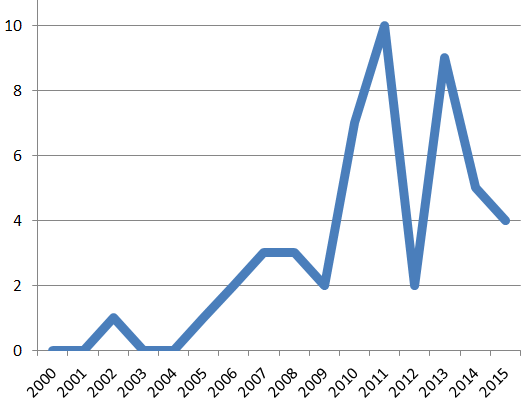
\includegraphics[scale=0.6]{PublicacionesAnuales.png}
  \end{center}
  \caption{Distribución de las publicaciones por años}
  \label{fig:PublicacionesAnuales}
\end{figure}

\subsection{Categorización del estudio}

Una vez revisados todos los artículos, se han extraído unas características o categorías comunes a la tipología de los trabajos. Todos los trabajos seleccionados hacen uso de algún tipo de software o metodología para evaluar algún tipo de competencia genérica. Sólo dos trabajos mencionan un enfoque como el que se propone en la introducción de este capítulo, es decir, aprovechando los registros de interacción de los estudiantes con el LMS como indicadores del desempeño de las competencias genéricas. Encontramos trabajos que se apoyan en la tecnología para el tratamiento o evaluación de las competencias, pero que terminan delegando parte de esta evaluación en el alumnado, ya sea mediante autoevaluación o evaluación entre iguales. Otros trabajos se basan en videojuegos o en las redes sociales para evaluar alguna competencia, mientras que otros desarrollan algún tipo de software o técnica. Finalmente hay algunos trabajos que simplemente detectan en su entorno la necesidad de la evaluación de las competencias de manera automática porque su forma de hacerlo les ocasiona una serie de problemas o desventajas con respecto a otro método que proponen o demandan. Además se han encontrado algunas revisiones sobre la literatura relacionadas que también serán tratadas aparte.  En la tabla \ref{tab:PublicacionesForum} se puede ver la distribución de las publicaciones. Algunos trabajos utilizan más de un método simultáneamente. %, apoyadas gráficamente en la figura  \ref{fig:PublicacionesForum}.

\begin{table}
  \begin{center}
  \begin{tabular}{| m{10cm} | c |}
    \hline
    CATEGORÍA & TRABAJOS\\
    \hline
    \hline 
    Peer and self-assessment & 18\\
    \hline
    Teacher assessment & 21\\
    \hline
    Questionaries & 16\\
    \hline
    Learning Analytics & 2\\
    \hline
  \end{tabular}
\end{center}
\caption{Distribución de publicaciones por tratamiento del problema}
\label{tab:PublicacionesForum}
\end{table} 

%\begin{figure}
%  \begin{center}
%    \includegraphics[scale=0.4]{cap3_pub_forum.png}
%  \end{center}
%  \caption{Distribución de publicaciones por tratamiento del problema}
%  \label{fig:PublicacionesForum}
%\end{figure}

En la figura \ref{fig:Burble} se muestra la clasificación de los trabajos según su ámbito y su tipo (lado izquierdo), y según su ámbito y su contribución (lado derecho). La evaluación de competencias genéricas mediante el uso de las nuevas tecnologías es un tema poco desarrollado. No sólo corroborado porque hay pocos trabajos, si no también a partir de esta figura. La mayoría de los trabajos son propuesta s(\emph{Proposal of solution}), experiencias (\emph{Experience papers}), validaciones (\emph{Validation research}) y evaluaciones de la investigación (\emph{Evaluation research}), mientras que trabajos de opinión(\emph{Opinion papers}) o filosóficos (\emph{Philosophical papers}), trabajos típicos de un tema de investigación de cierta madurez, casi no hay.

El tipo de contribución está más distribuído. Las contribuciones del tipo proceso (\emph{Process}) y modelo (\emph{Model}) son las que se dan con más frecuencia, la primera con cuestionarios (\emph{Questionnarie}), evaluación del profesores (\emph{Teacher assessment}) y autoevaluaciones o evaluaciones entre compañeros (\emph{Peer and self-assessment}), mientras que la segunda se da con más frecuencia con cuestionarios y evaluaciones del profesor. 

\pagestyle{empty}
\begin{landscape}
\begin{figure}[H]
  \begin{center}
    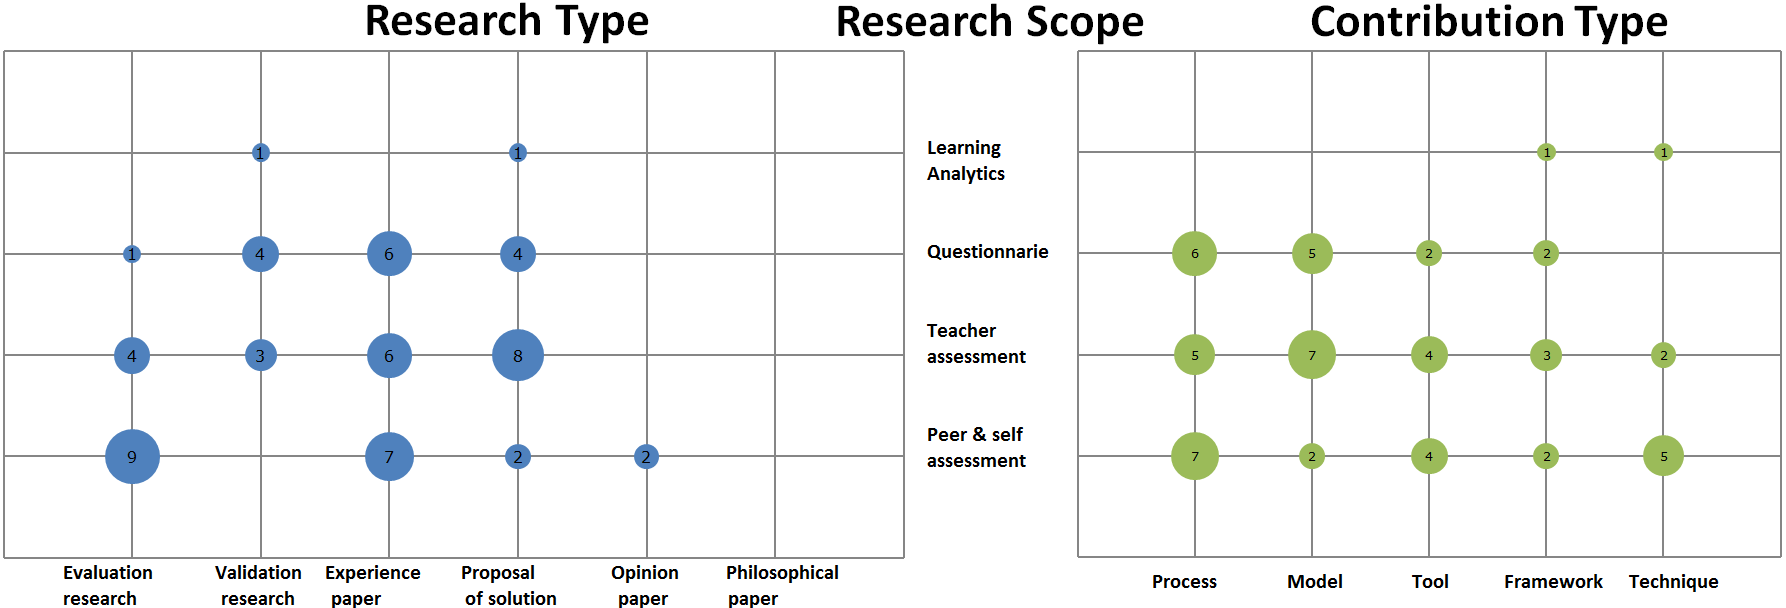
\includegraphics[scale=0.4]{Burbujas.png}
  \end{center}
  \caption{Ámbito de trabajos distribuidos según tipo de investigación y según tipo de contribución.}
  \label{fig:Burble}
\end{figure}
\end{landscape}
\pagestyle{fancy}

\subsection{Esquema de clasificación}

bla bla bla

\subsubsection{Peer and self-assessment}

La autoevaluación es un proceso en el que los estudiantes evaluan su propio trabajo, mientras que  en el proceso de evaluación entre iguales un estudiante evalúa el trabajo de otro u otros estudiantes. Esta práctica se emplea por un lado para ahorrar tiempo del profesorado, y por otro, para mejorar tanto el conocimiento en la materia del alumnado como sus habilidades metacognitivas. A menudo este tipo de evaluación se acompaña de algun tipo de rúbrica \cite{malehorn1994ten}.

Se han encontrado muchos trabajos en la literatura que utilizan este enfoque para evaluar competencias genéricas. De acuerdo a las preguntas de investigación de este trabajo únicamente se hanrecopilado aquellos trabajos que bajo este enfoque hagan uso de los ordenadores.

Se han encontrado varios trabajos que implementan una metodología de \emph{aprendizaje basado en problemas} (ABP o, del inglés, PBL, problem-based learning) para desarrollar competencias específicas y genéricas en sus estudiantes. En \cite{lasa2013problem} los profesores llevaron a cabo la evaluación del 90\% de las competencias utilizando la herramienta de rúbricas \emph{RubiStar}, mientras que los estudiantes mediante autoevaluación y evaluación entre iguales se encargaron del otro 10\%. En \cite{renau2010teaching} también se lleva a cabo una experiencia basada en una metodologia ABP para el desarrollo de la competencia en \emph{lengua extranjera} (inglés) en la que los estudiantes llevaban a cabo una autoevaluación de su nivel de adquisición de la competencia. En \cite{johnson2002encouraging} se muestran ejercicios para el desarrollo de competencias genéricas relacionados también con otra experiencia basada en una metodologia ABP y en unas presentaciones, siguiendo un enfoque de evaluaciones entre compañeros. En otro trabajo, vemos como los estudiantes después de haber realizado experiencias de videoconferencias en inglés, la competencia de \emph{inglés como lengua extranjera} junto con las competencias de \emph{trabajo en equipo} y \emph{comunicación oral} se evalúan en \cite{masip2013self} mediante auto y co-evaluación a través de Moodle.

El espíritu empresarial es considerado un factor fundamental para el desarrollo económico en todos los países del mundo \cite{DeXena2012educacion} y son muchos los trabajos que tratan de fomentar competencias genéricas relacionadas con las habilidades que un emprendedor ha de desempeñar. En \cite{chang2009international} se utiliza la herramienta Cycloid para el desarrollo de competencias en la gestión de proyectos y porteriormente se llevan a cabo autoevaluaciones de los propios estudiantes para valorar la adquisición de dichas competencias. En \cite{marquez2010have} se autoevalúan las competencias de \emph{iniciativa} y \emph{espíritu emprendedor}. También se autoevaluan competencias \emph{empresariales} en  \cite{achcaoucaou2014competence} mediante el uso de Tricuspoid. 

Un e-portfolio (del inglés \emph{electronic portfolio}, consiste en un conjunto de documentos, generalmente textos, archivos e imágenes, gestionados en un entorno web por un usuario. Se han recopilado trabajos donde los estudiantes trabajan con esta herramienta durante el curso y al final autoevalúan el desempeño de alguna competencia genérica. Por ejemplo, en \cite{arno2011promoting} se lleva a cabo una autoevaluación de la competencia del \emph{pensamiento crítico} tras haber trabajado en un e-portfolio. Mientras que en \emph{starcic2008sustaining} se utiliza también un e-portfolio para el desarrollo profesional de los estudiantes y se facilitan rubricas para la propia autoevaluación después de sus competencias genéricas.

En muchos trabajos la autoevaluación completa algún otro tipo de evaluación. En \cite{sevilla2012assessment} se utiliza plataforma online inGenio Tester para evaluar el nivel de adquisición de competencias en las modalidades de autoevaluación y evaluación por parte del profesor. En \cite{ficapal2015learning} se presenta un modelo que persigue el aprendizaje basado en equipos para la adquisición y evaluación de competencias genéricas en un contexto de e-learning. Los estudiantes trabajaban en grupo y evaluaban su desempeño en el \emph{trabajo en equipo} mediante una rúbrica. La calificación se completó con un cuestionario. En \cite{khamis2012measurement} también se trabajó y evaluó la competencia de \emph{trabajo en equipo}. Para ello los estudiates trabajaron en equipo y la evaluación tenía dos partes: por un lado los compañeros eran evaluados por otros compañeros (evaluación entre iguales) y por otro lado, también el profesor formaba parte de esta evaluación. En \cite{barbera2011assessment} se desarrollan y evalúan el desarrollo y desempeño de tres competencias genéricas en sus estudiantes: \emph{comunicación verbal}, \emph{comunicación escrita} y \emph{trabajo en equipo}. Este estudio propone una metodología basada en el modelo de tres niveles de evaluación de competencias utilizado por la Universidad de Deusto mediante diferentes herramientas utilizando tres tipos de evaluaciones: autoevaluación, evaluación entre iguales y evaluación del profesor.

En \cite{ruizacarate2013soft} los estudiantes responden a un cuestionario llamado \emph{Evalsoft} dónde son evaluados de las siguientes habilidades sociales: \emph{compromiso}, \emph{comunicación} y \emph{trabajo en equipo}. Para saber si el contexto es importante (online o presencial), se realiza en dos universidades: la Universidad a Distancia de Madrid (UDIMA), que ofrece un entorno de aprendizaje-enseñanza online y la Universidad Politécnica de Madrid (UPM), que además ofrece clases presenciales. Los resultados muestran que en un contexto online los estudiantes muestran un grado más alto de \emph{compromiso} y de \emph{trabajo en equipo}. Las herramientas 2.0 como wikis o blogs también se utilizan para medir el desempeño en competencias genéricas. En \cite{piedra2010measuring} se utilizan una serie de rúbricas para la autoevaluación de los estudiantes a partir de una serie de indicadores del desempeño de las competencias genéricas de la \emph{creatividad} y del \emph{trabajo colaborativo} a partir de su trabajo en herramientas de trabajo colaborativo. En \cite{mcloughlin2006beyond} se presentan una revisión de herramientas online para trabajar y evaluar competencas genéricas. Entre ellas también se mencionan herramientas colaborativas para la competencia del \emph{trabajo en equipo}. 

Para la evaluación de la competencia de la capacidad \emph{autocrítica} se realizó una experiencia en \cite{pinto2011assessment}, dónde un conjunto de profesores de diferentes titulaciones establecieron actividades para los estudiantes. Estos estudiantes evaluaron su propio trabajo. Para medir el grado de competencia de los estudiantes se utilizó la diferencia de la nota entre la que recibieron los estudiantes por parte del profesor y la que ellos mismos se pusieron. En \cite{sin2007evaluating} también se realizó una experiencia donde tanto los propios estudiantes como los profesores evaluaban el desempeño de las competencias de la comunicación en contabilidad, tanto las \emph{habilidades para expresarse de manera escrita} como del \emph{pensamiento analítico}.

Para conocer el nivel de adquisición de competencias genéricas que poseen los estudiantes que acceden a la universidad y enfocándose en las diferencias entre los estudiantes de ciencias y los que no son de ciencias, se propone en \cite{so2011mapping} un cuestionario de autoevaluación. Aunque la autoevaluación y evaluación entre iguales son enfoques que quitan trabajo al docente, no todos son ventajas. Como se ha visto en algunos trabajos anteriores, este enfoque a menudo sólo se utiliza de manera complementaria a algún otro tipo de evaluación. Además, se puede dar el caso que la autoevaluación no se ajuste del todo a la realidad del desempeño del estudiante. Por ejemplo, en \cite{carreras2013promotion} hay notables diferencias entre las calificaciones que se auto-asignan los estudiantes en algunas competencias y las calificaciones que le asignaron los profesores en esas mismas competencias. En ese trabajo se promovió la adquisición de competencias genéricas desde un punto de vista interdisciplinar y se diseñaron herramientas especifícas para evaluar dichas habilidades. A la hora de evaluar, se realizaron tanto autoevaluaciones como evaluaciones del profesor. En esta experiencia se evaluaron cuatro competencias genéricas: \emph{capacidad de análisis},  \emph{habilidades de escritura}, \emph{responsabilidad} y \emph{capacidad de trabajo en equipo}. Cabe destacar discrepancias entre las calificaciones que se auto-asignan los estudiantes en las dos primeras competencias. En la \emph{capacidad de análisis} la discrepancia es de un 55,65\%, mientras que en las \emph{habilidades de escritura} de un 13,75\%.



\subsubsection{Teacher assessment}

En muchos casos la evaluación de competencias genéricas se realiza mediante un seguimiento continuo del trabajo del estudiante por parte del profesor. Este proceso es lo que se conoce como \emph{evaluación continua}. Esto permite ir introduciendo mejoras constantes en el proceso de aprendizaje, siendo éste el motivo por el que la evaluación continua se adopta como una estrategia de evaluación formativa más orientada al proceso de aprendizaje que a una valoración puntual. Actualmente, los expertos, influenciados por la \emph{Declaración de Bolonia}, consideran más apropiado desarrollar este tipo de sistemas de evaluación~\cite{garcia2005competencias}. 

En trabajos como los mostrados en \cite{martin2010new,prashar2010competence}, el profesorado sigue una metodología de evaluación continua para evaluar las competencias de \emph{trabajo en equipo} y \emph{comunicación oral y escrita}. Se establecen una serie de indicadores que les permiten monitorizar el progreso de los estudiantes. Una herramienta que se suele utilizar para hacer un seguimiento del trabajo de los estudiantes a lo largo del curso es el e-portfolio. En \cite{martin2013acquired,rodriguez2010portfolio,benlloch2007adapting} los profesores evalúan el desempeño de los estudiantes en las competencias de \emph{trabajo en equipo} y \emph{habilidades de comunicación} o \emph{solución de problemas}, entre otras. Para ello utilizan el e-portfolio, aunque en todos los casos combinan la evaluación del trabajo realizado por cada estudiante en el suyo junto con la calificaciones de otras actividades, exámenes y cuestionarios.

En \cite{yang2014fine} se define un modelo de itinerario de aprendizaje que soporta la evaluación de algunos conocimientos y competencias para describir el progreso de aprendizaje del estudiante. El modelo se define matemáticamente para poder formalmente definir las evaluaciones y para poder reutilizar las fórmulas. Aunque se reconoce las ventajas de un sistema que automatice este proceso, hasta el momento son los profesores los que evalúan a sus estudiantes en cada una de sus etapas. Además, muestran su reticencia a un sistema 100\% automático. Las competencias de \emph{comunicación} y \emph{escritura} se evalúan en este trabajo.

Uno de los problemas de la no automatización de los procesos de evaluación es la escalabilidad de algunos procesos de evaluación. En \cite{serrano2013hiperion} se diseña \emph{Hiperion}, una sistema de recomendación que ayuda a diseñar actividades adaptadas a cada estudiante para mejorar sus competencias. En el estudio de caso mostrado en este trabajo, los profesores evaluaban las competencias de los estudiantes manualmente y después aplicaban Hiperion. La principal desventaja de la herramienta es el tiempo que el profesor ha de dedicar para asignar los diferentes logros y el peso de cada nota para cada competencia en las actividades. En \cite{ward2011developing} se desarrollan una serie de módulos para Moodle para el desarrollo de competencias empresariales. Los alumnos realizan una serie de actividades para cada módulo y el profesor evalúa mediante conferencia via Skype si cada estudiante sabe lo que ha respondido. En \cite{lacuesta2009active} se utiliza una metodología ABP, dónde se realiza una evaluación individualizada de cada estudiante y de cada grupo de estudiantes. El autor considera que el esfuerzo necesario y carga de trabajo para cada profesor sólo es un poco mayor al habitual. En este trabajo se evaluan competencias como la \emph{capacidad critica}, \emph{trabajo en equipo}, \emph{planificación}, \emph{comunicación}, etc. Para minimizar el esfuerzo están las rúbricas, utilizadas en \cite{casan2015developing}, donde el docente se encarga mediante su uso de la evaluación en las habilidades de \emph{comunicación escrita} del alumnado.

\subsubsection{Questionnarie}

Algunos de los cuestionarios que se han encontrado dentro de la bibliografia son tests de personalidad. Este tipo de cuestionario está diseñado para revelar aspectos del carácter o mecanismos psicológicos de un individuo. La evaluación de la personalidad se puede ver como la aplicación de procedimientos para medir aspectos de la personalidad de manera que sean aplicables a otros dominios~\cite{wiggins2003paradigms}. Uno de esos dominios es el laboral, sobre todo las entrevistas de trabajo. Es común la necesidad del empresario por conocer la aptitud o no del candidato a un puesto para asumir cierto rol dentro de una empresa. En \cite{andre2011formal} se propone un modelo formal para asignar trabajadores a proyectos software. Para definir el modelo se siguió un método Delphi, donde los expertos definieron criterios para la evaluación de habilidades de trabajo en equipo y definieron un test psicológico. Este modelo se plasmó en un software, que a partir de las respuestas del usuario, le asignaba un rol u otro dentro de los equipos. En \cite{lumsden2005assessment} se muestra la herramienta PQA (Personal Quality Assessment). Esta herramienta de evaluación contiene diversos test para la evaluación de la competencia genérica del \emph{razonamiento} y del {comportamiento ético} en el ámbito médico. En \cite{park2006moral} se muestra VIA-Youth (Values in Action Invetory for Youth) un cuestionario para evaluar la competencia \emph{moral} de los estudiantes a partir de preguntas relacionadas con 24 características de la personalidad. 

Las habilidades que hacen al individuo apto para el trabajo en equipo también son de las más medidas via cuestionarios. Según~\cite{martinez2014teamwork}, para obtener un buen desempeño en las competencias de trabajo en equipo hay que entrenarlas. Para contrastar su hipótesis, llevan a cabo un experimento donde se evalúa la competencia de \emph{trabajo en equipo} mediante el TWBQ (Team Work Behaviour Questionnaire). TWBQ es un cuestionario que evalua actividades individuales que contribuyen al devenir del equipo: por un lado, \emph{interacción con los compañeros}: conflictos y solución de problemas, colaboración, comunicación; y por otro lado \emph{gestión del equipo}: liderazgo, establecimiento de objetivos, planificación de taras, coordinación con los miembros del equipo). En \cite{barbera2011design} se lleva a cabo una experiencia en la que se aplicó una metodología ABP en la asignatura de Gestión de Empresas. Trabajaron las competencias de \emph{trabajo en equipo}, \emph{desarrollo de proyecto} y \emph{comunicación oral}. Para asegurar la objetividad de la evaluación se utilizaron rúbricas y cuestionarios. El profesorado que participó en la experiencia la consideró como muy positiva, pero reconocieron que tuvieron que dedicar un elevado número de horas, tanto para las clases como para la evaluación de muchos proyectos.

En \cite{badcock2010developing} se evaluan cuatro competencias genéricas: \emph{pensamiento crítico}, \emph{habilidades interpersonales}, \emph{solución de problemas} y \emph{comunicación escrita}. Para ello se utiliza el test GSA (Graduate Skills Assessment). El GSA fue desarrollado por el ACER (Australian Council for Educational Research)~\footnote{http://www.acer.edu.au/gsa}  bajo su Programa de Innovación para la Educación Superior. El objetivo con el que se diseñó es el de evaluar estas competencias genéricas cuando los estudiantes acceden a la universidad. Esto ayuda al profesorado a tener una medida objetiva para dichas competencias. Otro trabajo se muestra en~\cite{fernandez2011experience}, dónde se realiza un experimento en el que se presenta un test para evaluar la competencia de \emph{comunicación en un segundo idioma}, en este caso en inglés. En \cite{aziz2007appraisal,rashid2008engineering,a2007outcome} se utilizan modelos matemáticos (\emph{Rasch model} y \emph{ESPEGS model}) para la evaluación de los objetivos de aprendizaje del curso y de competencias genéricas. La entrada de estos modelos matemáticos son la evaluación de los estudiantes realizadas por los docentes para cada actividad. 

Los cuestionarios pueden constar de preguntas abiertas o cerradas. Las preguntas abiertas obligan al evaluado a formular la respuesta a la pregunta y al evaluador a leerla para corregirla, lo que conlleva una mayor carga de trabajo. En \cite{albergaria2011critical} se presenta un cuestionario para evaluar el \emph{pensamiento crítico}, la \emph{curiosidad} y la\emph{creatividad}. El cuestionario consta sobre todo de preguntas abiertas, lo que implica tener que dedicar más tiempo y recursos para realizar las evaluaciones. En \cite{vizcarro2013assessment}, profesores de los grados de Computación y Matemáticas y de Ingeniería Informática elaboraron una prueba escrita para la evaluación de la competencia genérica de \emph{resolución de problemas}. Este constaba de preguntas abiertas y cerradas, siendo minuciosamente por el profesorado que formaba parte en la experiencia, así como las respuestas que se esperarían de los estudiantes. El proyecto fue muy satisfactorio, aunque en las conclusiones vemos que los autores indican que encontrar un equilibrio entre el esfuerzo necesario para desarrollar este tipo de dispositivos de evaluación y la posibilidad de no hacerlo, o hacerlo pero no tan exhaustivamente, es algo que la comunidad académica debe abordar seriamente.

\subsubsection{Learning Analytics}


% JUEGOS SERIOS BASADOS EN INDICADORES: ¿LOS SACO DE LA?

En \cite{guenaga2013serious} se utilizan los juegos serios para el desarrollo de las competencias de \emph{emprendimiento} y \emph{solución de problemas}. Se definieron una serie de indicadores para alcanzar  que se plasmaron en un juego que permite al estudiante conocer su nivel de adquisición en dichas competencias.

En \cite{bedek2011behavioral} también se utilizan los juegos serios para el desarrollo y evaluación de competencias genéricas. Se basa en un modelo donde para casa competencia se identifican subcompetencias más específicas, lo que facilita el proceso de definición de indicadores.

Trabajos: \cite{fidalgo:2015} and \cite{rayon2014web}

\section{Respuestas}


%\chapter{Trabajo en curso y futuro}

\section{Conclusiones}

\pagestyle{empty}
\begin{landscape}
\begin{center}
\begin{longtable}{| m{2.5cm} | m{9cm} | m{4cm} | m{2.5cm} | m{3.5cm} |}
    \hline
    REF & TÍTULO & TIPO DE INVESTIGACIÓN & TIPO DE CONTRIBUCIÓN & ÁMBITO DE LA INVESTIGACIÓN \\
    \hline
    \hline 
    \cite{yang2014fine} & A Fine-Grained Outcome-Based Learning Path Model & proposal of solution & model & Teacher assessment \\
    \hline
    \cite{rayon2014web} & A web platform for the assessment of competences in Mobile Learning Contexts & validation research & framework & Learning analytics \\
    \hline
    \cite{martin2013acquired} & Acquired Skills With The Implementation Of New Evaluation Methods At University Rey Juan Carlos & experience paper & model & Teacher assessment \\
    \hline
    \cite{lacuesta2009active} & Active learning through problem based learning methodology in engineering education & experience paper & process & Teacher assessment \\
    \hline
    \cite{benlloch2007adapting} & Adapting teaching and assessment strategies to enhance competence-based learning in the framework of the european convergence process & proposal of solution & process & Teacher assessment / Questionnarie \\
    \hline
    \cite{aziz2007appraisal} & Appraisal of Course Learning Outcomes using Rasch Measurement: A Case Study in Information Technology Education & proposal of solution & model & Questionnarie / Teacher assessment \\
    \hline
    \cite{sevilla2012assessment} & Assessment of competences in designing online preparatory materials for the Cambridge First Certificate in English examination & evaluation research & technique & Peer and self-assessment / Teacher assessment \\
    \hline
    \cite{lumsden2005assessment} & Assessment of personal qualities in relation to admission to medical school & evaluation research & framework & Questionnarie \\
    \hline
    \cite{vizcarro2013assessment} & Assessment of problem solving in computing studies & experience paper & process & Questionnarie \\
    \hline
    \cite{pinto2011assessment} & Assessment Of Self-Criticism Capacity Competence In Higher Education Students: Outcome Oriented Education & experience paper & process & Peer and self-assessment \\
    \hline
    \cite{barbera2011assessment} & Assessment Tools For The Evaluation Of Generic Skills Development In Students Of Business Management & proposal of solution & model & Teacher assessment \\
    \hline
    \cite{mcloughlin2006beyond} & Beyond marks and measurement: Developing dynamic and authentic forms of e-assessment & opinion paper & technique & Peer and self-assessment \\
    \hline
    \cite{achcaoucaou2014competence} & Competence Assessment in Higher Education: A Dynamic Approach & proposal of solution & tool & Peer and self-assessment \\
    \hline
    \cite{prashar2010competence} & Competence Based Teaching And Evaluation In The General Chemistry Course Of The University Rey Juan Carlos & experience paper & framework & Teacher assessment \\
    \hline
    \cite{strijbos2015criteria} & Criteria and standards of generic competences at bachelor degree level: A review study & evaluation research & process & Pending \\
    \hline
    \cite{albergaria2011critical} & Critical Thinking, Questioning and Creativity as Components of Intelligence & proposal of solution & process & Questionnarie \\
    \hline
    \cite{barbera2011design} & "Design And Results Of Collaborative Project-Based Learning In The Subject Commercial Management"" In Industrial Organization Engineering""" & experience paper & framework & Questionnarie \\
    \hline
    \cite{ward2011developing} & Developing entrepreneurial accounting and finance competency using the ELLEIEC Virtual Centre for Enterprise & experience paper & tool & Teacher assessment \\
    \hline
    \cite{badcock2010developing} & Developing generic skills through university study: a study of arts, science and engineering in Australia & experience paper & model & Questionnarie \\
    \hline
    \cite{casan2015developing} & Developing Writing Skills in The Classroom: A Corpus-based Analysis of Multi-Genre Structures & proposal of solution & model & Teacher assessment \\
    \hline
    \cite{ficapal2015learning} & e-Learning and Team-based Learning. Practical Experience in Virtual Teams & experience paper & framework & Peer and self-assessment / Questionnarie \\
    \hline
    \cite{johnson2002encouraging} & Encouraging generic skills in science courses & proposal of solution & process & Peer and self-assessment / Teacher assessment \\
    \hline
    \cite{rashid2008engineering} & Engineering Students Performance Evaluation of Generic Skills Measurement: ESPEGS Model & validation research & model & Questionnarie / Teacher assessment \\
    \hline
    \cite{rodriguez2010portfolio} & e-Portfolio: A tool to assess university students' skills & evaluation research & tool & Teacher assessment \\
    \hline
    \cite{sin2007evaluating} & Evaluating a method of integrating generic skills with accounting content based on a functional theory of meaning & evaluation research & process & Peer and self-assessment / Teacher assessment \\
    \hline
    \cite{andre2011formal} & Formal model for assigning human resources to teams in software projects & validation research & model & Questionnarie \\
    \hline
    \cite{bedek2011behavioral} & From Behavioral Indicators to Contextualized Competence Assessment & proposal of solution & framework & Teacher assessment \\
    \hline
    \cite{oliver2013graduate} & Graduate attributes as a focus for institution-wide curriculum renewal: innovations and challenges & opinion paper & model & Peer and self-assessment \\
    \hline
    \cite{marquez2010have} & Have Our Future Entrepreneurs An Ethical Commitment? & evaluation research & process & Peer and self-assessment \\
    \hline
    \cite{serrano2013hiperion} & Hiperion: A fuzzy approach for recommending educational activities based on the acquisition of competences & proposal of solution & tool & Teacher assessment \\
    \hline
    \cite{chang2009international} & International creative tension study of university students in South Korea and Finland & evaluation research & tool & Peer and self-assessment \\
    \hline
    \cite{} & Making Explicit and Reinforcing Horizontal Competences in an Electronic Engineering Degree & validation research & process & Teacher assessment \\
    \hline
    \cite{so2011mapping} & Mapping The Impact On Holistic Development: A Study Of The Relationship & proposal of solution & process & Questionnarie \\
    \hline
    \cite{khamis2012measurement} & Measurement of Students' Performance Level in a Group Project by using Peer Review and Lecturer Assessment & experience paper & technique & Peer and self-assessment / Teacher assessment \\
    \hline
    \cite{piedra2010measuring} & Measuring collaboration and creativity skills through rubrics: Experience from UTPL collaborative social networks course & evaluation research & process & Peer and self-assessment \\
    \hline
    \cite{park2006moral} & Moral competence and character strengths among adolescents: The development and validation of the Values in Action Inventory of Strengths for Youth & validation research & tool & Questionnarie \\
    \hline
    \cite{martin2010new} & New Methodologies In The Teaching And Evaluation Of The Competences “Teamwork” And “Oral And Written Communication” In The Civil Law Course Of The University Rey Juan Carlos & experience paper & framework & Teacher assessment \\
    \hline
    \cite{a2007outcome} & Outcome based education performance assessment: A computational model to measure electrical engineering subjects learning outcomes & evaluation research & model & Questionnarie /Teacher assessment \\
    \hline
    \cite{lasa2013problem} & Problem Based Learning Implementation In The Degree Of Human Nutrition And Dietetics & experience paper & technique & Peer and self-assessment / Teacher assessment \\
    \hline
    \cite{arno2011promoting} & Promoting reflection on science, technology, and society among engineering students through an EAP online learning environment & evaluation research & tool & Peer and self-assessment \\
    \hline
    \cite{masip2013self} & Self-video recording for the integration and assessment of generic competencies & experience paper & technique & Peer and self-assessment \\
    \hline
    \cite{guenaga2013serious} & Serious Games for the Development of Employment Oriented Competences & validation research & tool & Teacher assessment \\
    \hline
    \cite{ruizacarate2013soft} & Soft Skills: A Comparative Analysis Between Online and Classroom Teaching & experience paper & process & Questionnarie \\
    \hline
    \cite{starcic2008sustaining} & Sustaining Teacher's Professional Development and Training through Web-Based Communities of Practice & evaluation research & tool & Peer and self-assessment \\
    \hline
    \cite{renau2010teaching} & Teaching And Learning Through Projects Using The ICT: Practice Of The English Writing Through Business Documents & experience paper & process & Peer and self-assessment \\
    \hline
    \cite{martinez2014teamwork} & Teamwork competence and academic motivation in computer science engineering studies & validation research & process & Questionnarie \\
    \hline
    \cite{fernandez2011experience} & The experience of implementing a communication skills assessment in the first year course for undergraduate computing engineering students: A tool for further development of an international curriculum & experience paper & tool & Questionnarie \\
    \hline
    \cite{carreras2013promotion} & The promotion and assessment of generic skills from interdisciplinary teaching teams & experience paper & process & Peer and self-assessment / Teacher assessment \\
    \hline
    \cite{fidalgo:2015} & Using Learning Analytics to improve teamwork assessment & proposal of solution & technique & Learning analytics \\
    \hline
\caption{Distribución de publicaciones por tratamiento del problema}
\label{tab:ListadoTrabajos}
\end{longtable}
\end{center}
\end{landscape}

\pagestyle{fancy}


% ----------------------------------------------------------------------

